\problemname{Vasaloppet}
\noindent
Charlotte tittar på Vasaloppet på TV. Sändningen börjar vid sekund $0$ och slutar vid sekund $T$. Tyvärr finns det
också $N$ reklamavbrott, som varar under $N$ icke-överlappande intervall av sekunder mellan sekund $0$ och sekund $T$. 
Charlotte blir väldigt inspirerad av att se de tävlande på startlinjen, 
och vill därför själv ut och åka skidor under loppet.
Hennes skidtur tar $S$ sekunder, och för att se vem som vinner Vasaloppet måste hon vara tillbaka senast vid sekund $T$.

Charlotte vill åka på sin skidtur vid ett tillfälle då hon missar så lite av Vasaloppet som möjligt. Din uppgift
är att räkna ut det minsta antalet sekunder av Vasaloppet som Charlotte kan missa,
om hon optimalt väljer när hon ska åka på sin skidtur.
Missade sekunder är de sekunder när Charlotte är ute på sin skidtur samtidigt som det inte är reklampaus.

\begin{centering}
  \begin{figure}[h]
      \centering
      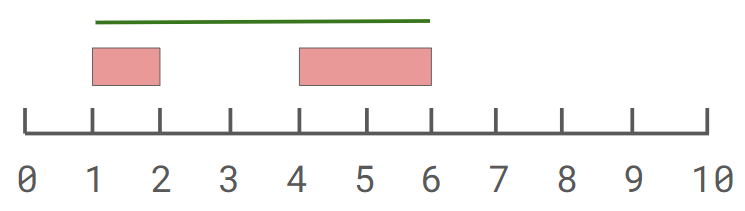
\includegraphics[width=0.6\textwidth]{sample1.PNG}
      \caption{Bilden föreställer första exempelfallet. De röda rektanglarna är reklampauserna. Om Charlotte börjar sin skidtur när första pausen börjar och kommer tillbaka när andra pausen slutar så missar hon bara $2$ sekunder av Vasaloppet.}
      \label{fig:enter-label}
  \end{figure}
\end{centering}

\section*{Indata}
Den första raden innehåller tre heltal $N,T$ och $S$ ($0 \leq N \leq 10^5$, $1 \leq S \leq T \leq 10^9$). 
$N$ är antalet reklamavbrott, $T$ sändningens längd i sekunder, och $S$ är längden på skidturen i sekunder.

Därefter följer $N$ rader som vardera innehåller två heltal $l_i, r_i$ ($0 \leq l_i < r_i \leq T$),
vilket betyder att det $i$:te reklamavbrottet varar från sekund $l_i$ till sekund $r_i$.\\
Reklamavbrotten ges även i samma ordning som de startar, och alla reklamavbrott är disjunkta och sorterade, 
det vill säga att $r_i < l_{i+1}$ för $i < N$. 

\section*{Utdata}
Skriv ut ett heltal, det minsta antalet sekunder som Charlotte kan missa av Vasaloppet under sin skidtur om den väljs optimalt. 
Notera att skidturen får sluta precis vid sekund $T$. 
Exempelvis kan skidturen vara under hela Vasaloppet om $S=3$ och $T=3$.

\section*{Poängsättning}
Din lösning kommer att testas på en mängd testfallsgrupper.
För att få poäng för en grupp så måste du klara alla testfall i gruppen.

\noindent
\begin{tabular}{| l | l | p{12cm} |}
  \hline
  \textbf{Grupp} & \textbf{Poäng} & \textbf{Gränser} \\ \hline
  $1$    & $10$       & $N=1$ \\ \hline
  $2$    & $25$       & $N \leq 1000$ \\ \hline
  $3$    & $30$       & $T \leq 10^6$ \\ \hline
  $4$    & $35$       & Inga ytterligare begränsningar. \\ \hline
\end{tabular}